%%%%%%%%%%%%%%%%%%%%%%%%%%%%%%%%%%%%%%%%%
% Short Sectioned Assignment LaTeX Template Version 1.0 (5/5/12)
% This template has been downloaded from: http://www.LaTeXTemplates.com
% Original author:  Frits Wenneker (http://www.howtotex.com)
% License: CC BY-NC-SA 3.0 (http://creativecommons.org/licenses/by-nc-sa/3.0/)
%%%%%%%%%%%%%%%%%%%%%%%%%%%%%%%%%%%%%%%%%

%----------------------------------------------------------------------------------------
%	PACKAGES AND OTHER DOCUMENT CONFIGURATIONS
%----------------------------------------------------------------------------------------

\documentclass[paper=a4, fontsize=11pt]{scrartcl} % A4 paper and 11pt font size

% ---- Entrada y salida de texto -----

\usepackage[T1]{fontenc} % Use 8-bit encoding that has 256 glyphs
\usepackage[utf8]{inputenc}
%\usepackage{fourier} % Use the Adobe Utopia font for the document - comment this line to return to the LaTeX default

% ---- Idioma --------

\usepackage[spanish, es-tabla]{babel} % Selecciona el español para palabras introducidas automáticamente, p.ej. "septiembre" en la fecha y especifica que se use la palabra Tabla en vez de Cuadro

% ---- Otros paquetes ----

\usepackage{amsmath,amsfonts,amsthm} % Math packages
%\usepackage{graphics,graphicx, floatrow} %para incluir imágenes y notas en las imágenes
\usepackage{graphics,graphicx, float} %para incluir imágenes y colocarlas

% Para hacer tablas comlejas
%\usepackage{multirow}
%\usepackage{threeparttable}

%\usepackage{sectsty} % Allows customizing section commands
%\allsectionsfont{\centering \normalfont\scshape} % Make all sections centered, the default font and small caps

\usepackage{fancyhdr} % Custom headers and footers
\usepackage{url}
\usepackage{hyperref}
\pagestyle{fancyplain} % Makes all pages in the document conform to the custom headers and footers
\fancyhead{} % No page header - if you want one, create it in the same way as the footers below
\fancyfoot[L]{} % Empty left footer
\fancyfoot[C]{} % Empty center footer
\fancyfoot[R]{\thepage} % Page numbering for right footer
\renewcommand{\headrulewidth}{0pt} % Remove header underlines
\renewcommand{\footrulewidth}{0pt} % Remove footer underlines
\setlength{\headheight}{13.6pt} % Customize the height of the header

\numberwithin{equation}{section} % Number equations within sections (i.e. 1.1, 1.2, 2.1, 2.2 instead of 1, 2, 3, 4)
\numberwithin{figure}{section} % Number figures within sections (i.e. 1.1, 1.2, 2.1, 2.2 instead of 1, 2, 3, 4)
\numberwithin{table}{section} % Number tables within sections (i.e. 1.1, 1.2, 2.1, 2.2 instead of 1, 2, 3, 4)

\setlength\parindent{0pt} % Removes all indentation from paragraphs - comment this line for an assignment with lots of text

\newcommand{\horrule}[1]{\rule{\linewidth}{#1}} % Create horizontal rule command with 1 argument of height

\usepackage{booktabs}




%----------------------------------------------------------------------------------------
%	TÍTULO Y DATOS DEL ALUMNO
%----------------------------------------------------------------------------------------

\title{	
\normalfont \normalsize 
\textsc{{\bf Aprendizaje Automático (2014-2015)} \\ Grado en Ingeniería Informática \\ Universidad de Granada} \\ [25pt] % Your university, school and/or department name(s)
\horrule{0.5pt} \\[0.4cm] % Thin top horizontal rule
\huge Práctica 2 \\ % The assignment title
\horrule{2pt} \\[0.5cm] % Thick bottom horizontal rule
}

\author{Ignacio Martín Requena} % Nombre y apellidos

\date{\normalsize\today} % Incluye la fecha actual

%----------------------------------------------------------------------------------------
% DOCUMENTO
%----------------------------------------------------------------------------------------
\usepackage{graphicx}
\usepackage{listings}
\usepackage{color}
\definecolor{gray97}{gray}{.97}
\definecolor{gray75}{gray}{.75}
\definecolor{gray45}{gray}{.45}
 

\lstset{ frame=Ltb,
     framerule=0pt,
     aboveskip=0.5cm,
     framextopmargin=3pt,
     framexbottommargin=3pt,
     framexleftmargin=0.4cm,
     framesep=0pt,
     rulesep=.4pt,
     backgroundcolor=\color{gray97},
     rulesepcolor=\color{black},
     %
     stringstyle=\ttfamily,
     showstringspaces = false,
     basicstyle=\small\ttfamily,
     commentstyle=\color{gray45},
     keywordstyle=\bfseries,
     %
     numbers=left,
     numbersep=15pt,
     numberstyle=\tiny,
     numberfirstline = false,
     breaklines=true,
   }
 


\lstdefinestyle{consola}
   {basicstyle=\scriptsize\bf\ttfamily,
    backgroundcolor=\color{gray75},
   }
 
\lstdefinestyle{C}
   {language=C,
   }



\begin{document}

\maketitle % Muestra el Título

\newpage %inserta un salto de página

\tableofcontents % para generar el índice de contenidos

\listoffigures

%\listoftables

\newpage



%----------------------------------------------------------------------------------------
%	Cuestion 1
%----------------------------------------------------------------------------------------

\section{Cuestionario}

\subsection{asdfas}


\subsubsection{asdfasdf}

\section{Ejercicios de implementacion}

%----------------------------------------------------------------------------------------
%	Cuestion 1
%----------------------------------------------------------------------------------------
\subsection{Usar la base de datos Weekly (ISLR) . Este conjunto de datos presenta predicciones semanales (1089) del mercado de valores durante 21 años (1990-2010).}

\subsubsection{Analizar la conducta de los datos usando resúmenes numéricos y gráficos de los mismos. ¿Se observa algún patrón de interés? En caso afirmativo dar una posible interpretación del mismo.}
Utilizando la función \emph{plot} de R podemos ver de un vistazo la relación que puede existir entre las variables denuestra base de datos:

\begin{figure}[H]
\centering
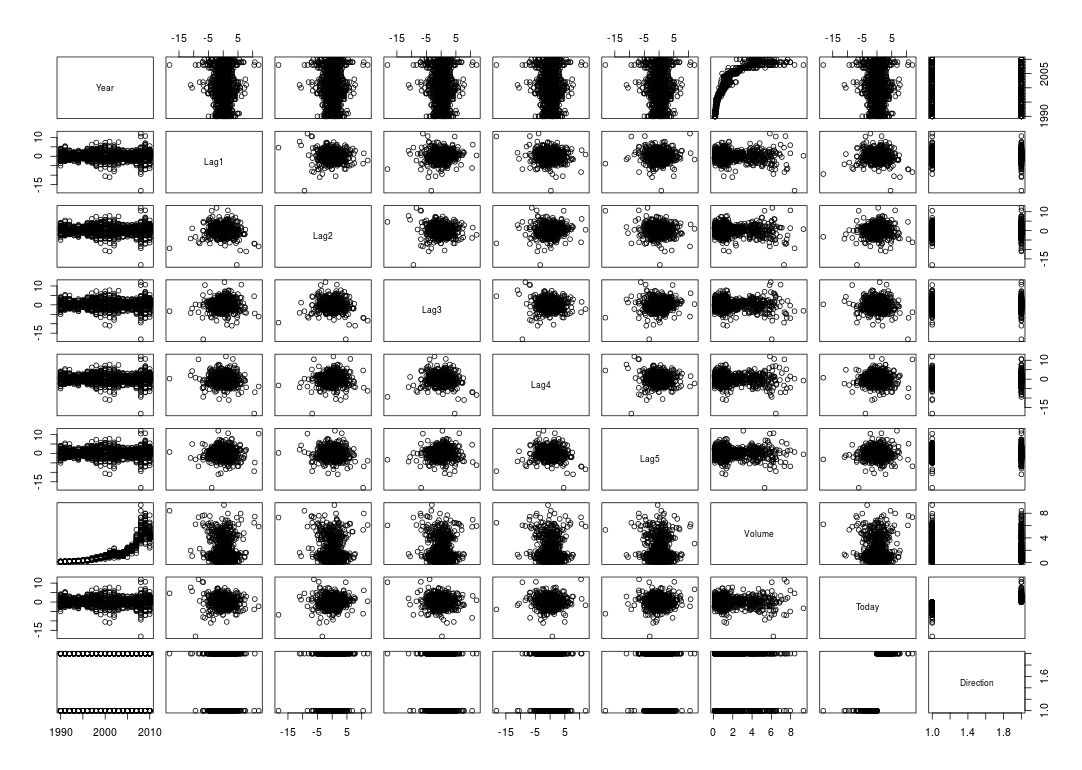
\includegraphics[scale=.40]{plot_weekly_all.png}
\caption{Representacion todas las variables}
\label{}
\end{figure}



\subsubsection{Usar la base de datos completa para ajustar un modelo de Regresión Logística usando Direction como variable respuesta y las variables Volume y Lag-1 a Lag-5 como predictores. Usar la función summary() para mostrar los resultados. ¿Alguno de los predictores es estadísticamente significativo? En caso afirmativo, ¿cuál? Justificar la respuesta}



\subsubsection{Calcular la matriz de confusión y el porcentaje total de predicciones correctas. Explicar lo que la matriz de confusión nos dice acerca de los errores cometidos por regresión logística. Justificar las respuesta}


\subsubsection{Ahora ajustar un modelo de regresión logística a los datos entre 1990 y 2008 usando Lag2 como el único predictor. Calcular la matriz de confusión y la fracción global de predicciones correctas para el periodo 2009 y 2010. Justificar las respuesta}

\subsubsection{Repetir (4) usando LDA, QDA y KNN con K=1. ¿Cuál de estos métodos parece dar los mejores resultados? Justificar las respuesta}


\subsubsection{Experimente con diferentes combinaciones de predictores, incluyendo transformaciones de las variables e interacciones entre ellas, en cada uno de los métodos (RLG, LDA, QDA, KNN) (si se desea, pueden usarse técnicas de selección de variables) . Muestre las variables, método y matriz de confusión que da los mejores resultados sobre los datos de test (2009-2010). Justificar las respuestas adecuadamente.}


\subsubsection{Repetir el punto anterior usando un modelo de ajuste de validación cruzada con 10 particiones. Comparar con los resultados obtenidos en el punto anterior. Justificar las respuestas adecuadamente.}


\end{document}